\section{鞍点}
\label{sec:minimax-saddle}

判断一个$\bm{x}$好不好，要算$\phi(\bm{x})$，也就要解一次内层。如果手上同时有一个$\bm{x}$和一个$\bm{y}$，能不能让它们互相作证？本节研究这样一对候选应当满足什么关系，它和两个次序的值有什么联系。

记交换次序后的函数为
\begin{equation}
 \psi(\bm{y})=\inf_{\bm{x}\in\bm{X}}f(\bm{x},\bm{y}),
 \label{eq:minimax-psi}
\end{equation}
它是$\bm{y}$先定时外层能做到的最好代价。两个次序的值分别记作
\begin{equation}
 \bar{v}=\inf_{\bm{x}\in\bm{X}}\phi(\bm{x}),\qquad\underline{v}=\sup_{\bm{y}\in\bm{Y}}\psi(\bm{y}).
 \label{eq:minimax-values}
\end{equation}
式~\eqref{eq:minimax-weak}就是$\underline{v}\leq\bar{v}$。

想象一个山口。沿着山脊方向，山口是最低点；沿着翻山的方向，山口是最高点。站在山口，往山脊两头走都要上坡，往两侧山谷走都要下坡。下面的定义把这个图景用到两组变量上：沿$\bm{x}$的方向山口最低，沿$\bm{y}$的方向山口最高。

\begin{definition}[全局鞍点]
\label{def:minimax-saddle}
若$(\bm{x}^\star,\bm{y}^\star)\in\bm{X}\times\bm{Y}$对所有$\bm{x}\in\bm{X}$，$\bm{y}\in\bm{Y}$满足
\begin{equation}
 f(\bm{x}^\star,\bm{y})\leq f(\bm{x}^\star,\bm{y}^\star)\leq f(\bm{x},\bm{y}^\star),
 \label{eq:minimax-saddle}
\end{equation}
就称它是$f$在$\bm{X}\times\bm{Y}$上的\term{全局鞍点}（global saddle point）。
\end{definition}

式~\eqref{eq:minimax-saddle}的右半边说，固定$\bm{y}^\star$时$\bm{x}^\star$全局最小；左半边说，固定$\bm{x}^\star$时$\bm{y}^\star$全局最大。任何一侧单独改变，都不能改善自己的目标。山口的类比在这里到头了：山的形状只有一种，而鞍点还取决于哪个变量要最小化、哪个要最大化。

这个定义比第~\ref{chap:saddle-points}章的鞍点多了分工。那一章的鞍点指Hessian不定的驻点，只看函数形状，不问变量的角色。

要把几个相近的概念分开，看图~\ref{fig:minimax-saddle-types}中的三个二次函数，以及后面一个四次函数。$x$是外层变量，$y$是内层变量。

\begin{BookInlineFigure}
 \centering
 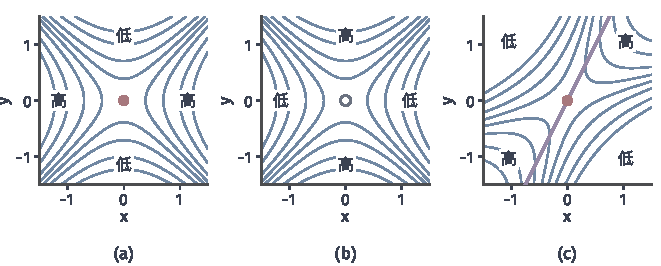
\includegraphics[width=112mm]{figures/05-optimization/07-multiple-criteria-and-nested-optimization/matplotlib/minimax-saddle-types/figure.pdf}
 \caption{原点都是两侧一阶驻定点，蓝线是等高线，“高”“低”标出函数值的高低区域。(a)$x^2-y^2$：沿$x$最小、沿$y$最大，红点是全局鞍点。(b)$y^2-x^2$：形状相同而角色相反，空心点既不是鞍点，也不解决顺序问题。(c)$-\frac12x^2+2xy-\frac12y^2$：紫线是最优响应$y=2x$，红点解决顺序问题，却不是鞍点。}
 \label{fig:minimax-saddle-types}
\end{BookInlineFigure}

(a)的$f=x^2-y^2$在全平面满足式~\eqref{eq:minimax-saddle}，原点是全局鞍点。(b)的$f=y^2-x^2$在原点的两个偏导数也都为零，但固定$y=0$时$-x^2$在$x=0$处最大，外层变量离开原点反而更好。

(c)最值得留意。取$f=-\frac12x^2+2xy-\frac12y^2$，$X=Y=\mathbb{R}$。这个函数在本章后面反复使用。内层关于$y$严格凹，令$\partial_yf=2x-y=0$，得$y^\star(x)=2x$。代回得到
\begin{equation}
 \phi(x)=-\frac12x^2+4x^2-2x^2=\frac32x^2.
 \label{eq:minimax-running-phi}
\end{equation}

$\phi$的最小点是$x=0$，顺序问题的解是原点，值是$0$。可是固定$y=0$时$f(x,0)=-\frac12x^2$在$x=0$处最大，式~\eqref{eq:minimax-saddle}的右半边不成立。对任意$y$，$\psi(y)=\inf_xf=-\infty$，所以$\underline{v}=-\infty<0=\bar{v}$。外层在这里不是对$\bm{x}$最小化固定的$f$，它考虑的是$y$会跟着$x$一起变，这个跟随效应把$-\frac12x^2$的向下弯曲翻了过来。

局部的版本是把式~\eqref{eq:minimax-saddle}中的“所有”改成“$(\bm{x}^\star,\bm{y}^\star)$某个邻域内的所有”，称为\term{局部鞍点}（local saddle point）。例如在$X=[-3,3]$，$Y=[-1,1]$上取
\begin{equation}
 f(x,y)=x^2-\frac14x^4-y^2.
 \label{eq:minimax-local-saddle}
\end{equation}
在原点附近$x^2-\frac14x^4\geq0$，所以原点是局部鞍点。但$f(3,0)=9-\frac{81}{4}=-11.25<0$，外层变量跑远了反而更好，所以原点不是全局鞍点。

\begin{BookInlineTable}
 \centering
 \begin{tabular}{@{}lll@{}}
  \toprule
  概念 & 要求 & 例子\\
  \midrule
  两侧一阶驻定 & 无约束时两个偏梯度为零 & 图~\ref{fig:minimax-saddle-types}三个原点\\
  局部鞍点 & 式~\eqref{eq:minimax-saddle}在邻域内成立 & 式~\eqref{eq:minimax-local-saddle}的原点\\
  全局鞍点 & 式~\eqref{eq:minimax-saddle}在全域成立 & $x^2-y^2$的原点\\
  顺序问题的解 & $\bm{x}$最小化$\phi$ & 图~\ref{fig:minimax-saddle-types}(c)的原点\\
  \bottomrule
 \end{tabular}
 \caption{四个相近概念的比较。两侧一阶驻定最弱，它不自动解决顺序问题；顺序问题的解也不一定是鞍点。}
 \label{tab:minimax-saddle-compare}
\end{BookInlineTable}

全局鞍点与两个次序的关系，由下面的定理给出。

\begin{theorem}[鞍点与最值相等]
\label{thm:minimax-saddle-values}
设$\bm{x}^\star\in\bm{X}$，$\bm{y}^\star\in\bm{Y}$。$(\bm{x}^\star,\bm{y}^\star)$是全局鞍点，当且仅当同时满足
\begin{equation}
 \phi(\bm{x}^\star)=\bar{v},\qquad\psi(\bm{y}^\star)=\underline{v},\qquad\bar{v}=\underline{v}\in\mathbb{R}.
 \label{eq:minimax-saddle-values}
\end{equation}
此时共同的值等于$f(\bm{x}^\star,\bm{y}^\star)$。
\end{theorem}

\begin{proof}
必要性。对式~\eqref{eq:minimax-saddle}的左半边取$\bm{y}$的上确界，右半边取$\bm{x}$的下确界，得到
\[
 \phi(\bm{x}^\star)\leq f(\bm{x}^\star,\bm{y}^\star)\leq\psi(\bm{y}^\star).
\]
结合定义，又有
\[
 \underline{v}\leq\bar{v}\leq\phi(\bm{x}^\star),\qquad\psi(\bm{y}^\star)\leq\underline{v}.
\]
把这些不等式连起来，就成为一个闭环，其中所有的量都相等。

充分性。由式~\eqref{eq:minimax-saddle-values}，$\phi(\bm{x}^\star)=\psi(\bm{y}^\star)$是有限数。定义给出
\[
 \psi(\bm{y}^\star)\leq f(\bm{x}^\star,\bm{y}^\star)\leq\phi(\bm{x}^\star),
\]
所以三者相等。于是对任意$\bm{x},\bm{y}$，
\[
 f(\bm{x}^\star,\bm{y})\leq\phi(\bm{x}^\star)=\psi(\bm{y}^\star)\leq f(\bm{x},\bm{y}^\star),
\]
中间的值等于$f(\bm{x}^\star,\bm{y}^\star)$，这就是式~\eqref{eq:minimax-saddle}。
\end{proof}

定理说明鞍点集合是一个乘积集合。若$(\bm{x}_1,\bm{y}_1)$和$(\bm{x}_2,\bm{y}_2)$都是鞍点，式~\eqref{eq:minimax-saddle-values}的三条对$(\bm{x}_1,\bm{y}_2)$同样成立，所以它也是鞍点，不需要把两侧配对寻找。这与第~\ref{chap:duality}章的Lagrange鞍点定理一致，那里的$\mathcal{L}$就是这里的$f$。

\subsection{最值交换}
\label{sec:minimax-exchange}

什么条件能让$\underline{v}=\bar{v}$？先回到图~\ref{fig:minimax-cost-table}的代价表，看一个修复办法。两个次序之所以不同，是因为每一方只能选一个端点。设想方案可以按比例组合：把份额$p$投给方案$\mathrm{a}$，$1-p$投给方案$\mathrm{b}$；扰动也按比例$q$和$1-q$作用，代价按份额加权。

记$p,q\in[0,1]$，代价为
\[
 f(p,q)=3pq+p(1-q)+2(1-p)(1-q).
\]
展开并配方，得到
\begin{equation}
 f(p,q)=4pq-p-2q+2=4\Bigl(p-\frac12\Bigr)\Bigl(q-\frac14\Bigr)+\frac32.
 \label{eq:minimax-relaxed}
\end{equation}

$f$关于$q$是线性的，最大值在端点取到，所以
\[
 \phi(p)=\max\{f(p,0),f(p,1)\}=\max\{2-p,3p\}.
\]
同理，$f$关于$p$线性，最小值在端点取到，所以
\[
 \psi(q)=\min\{f(0,q),f(1,q)\}=\min\{2-2q,1+2q\}.
\]

$\phi$在$2-p=3p$即$p=\frac12$处最小，$\psi$在$2-2q=1+2q$即$q=\frac14$处最大，并且
\[
 \phi\Bigl(\frac12\Bigr)=\psi\Bigl(\frac14\Bigr)=\frac32.
\]
由定理~\ref{thm:minimax-saddle-values}，$(\frac12,\frac14)$是鞍点，见图~\ref{fig:minimax-relaxed-table}。两个次序现在给出同一个值$\frac32$，它落在原来的$1$和$2$之间。允许按比例组合，也就是把问题做成关于各自变量线性的，先后的差别消失了。

\begin{BookInlineFigure}
 \centering
 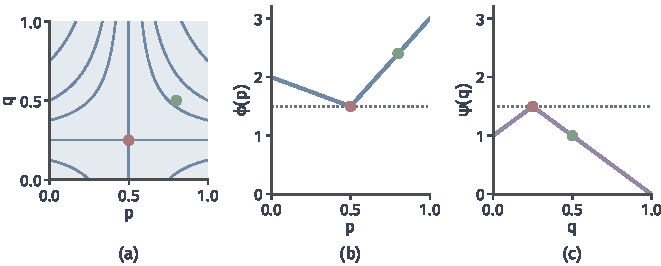
\includegraphics[width=112mm]{figures/05-optimization/07-multiple-criteria-and-nested-optimization/matplotlib/minimax-relaxed-table/figure.pdf}
 \caption{代价表的比例松弛$f(p,q)=4(p-\frac12)(q-\frac14)+\frac32$。(a)浅蓝是可行域，蓝线是等高线，穿过红点的十字是值为$\frac32$的等高线，红点是鞍点，绿点是候选$(0.8,0.5)$。(b)外层目标$\phi(p)$，红点是最小点。(c)$\psi(q)$，红点是最大点。点线是共同的值$\frac32$，绿点是候选在两条曲线上的值。}
 \label{fig:minimax-relaxed-table}
\end{BookInlineFigure}

这个例子的结构可以一般化：两个集合都是紧凸集，$f$关于$\bm{x}$凸、关于$\bm{y}$凹。凸凹性是说，混合之后不会比原来更有利于对面。

\begin{theorem}[紧集上的极小极大定理]
\label{thm:minimax-theorem}
设$\bm{X},\bm{Y}$非空、紧、凸，$f$在$\bm{X}\times\bm{Y}$上连续；对每个$\bm{y}\in\bm{Y}$，$f(\cdot,\bm{y})$是凸函数；对每个$\bm{x}\in\bm{X}$，$f(\bm{x},\cdot)$是凹函数。则
\begin{equation}
 \min_{\bm{x}\in\bm{X}}\max_{\bm{y}\in\bm{Y}}f(\bm{x},\bm{y})=\max_{\bm{y}\in\bm{Y}}\min_{\bm{x}\in\bm{X}}f(\bm{x},\bm{y}),
 \label{eq:minimax-theorem}
\end{equation}
两侧的最值都达到，并且存在全局鞍点。
\end{theorem}

\begin{proof}
由式~\eqref{eq:minimax-weak}，只需排除$\underline{v}<\bar{v}$。用反证法，设$\underline{v}<\bar{v}$，取实数$c$满足$\underline{v}<c<\bar{v}$。

第一步，把无穷多个$\bm{y}$化成有限个。对每个$\bm{x}\in\bm{X}$，有$\phi(\bm{x})\geq\bar{v}>c$，所以存在$\bm{y}$使$f(\bm{x},\bm{y})>c$。于是开集族
\[
 \bm{U}_{\bm{y}}=\{\bm{x}\in\bm{X}:f(\bm{x},\bm{y})>c\},\qquad\bm{y}\in\bm{Y}
\]
覆盖了$\bm{X}$。$\bm{X}$是紧集，存在有限个$\bm{y}_1,\ldots,\bm{y}_k$，使每个$\bm{x}\in\bm{X}$都至少满足一条$f(\bm{x},\bm{y}_i)>c$。

第二步，用凸性分离出权重。令
\[
 \bm{S}=\bigl\{\bm{w}\in\mathbb{R}^k:\text{存在}\ \bm{x}\in\bm{X},\ \text{使}\ w_i\geq f(\bm{x},\bm{y}_i)\ \text{对所有}\ i\ \text{成立}\bigr\}.
\]
$\bm{X}$是凸集，每个$f(\cdot,\bm{y}_i)$是凸函数，所以$\bm{S}$是凸集。点$\bm{c}=(c,\ldots,c)$不在$\bm{S}$中，否则某个$\bm{x}$使所有$f(\bm{x},\bm{y}_i)\leq c$，与第一步矛盾。

第~\ref{chap:duality}章的点与凸集分离引理不要求$\bm{S}$闭，由它得到$\bm{a}\neq\bm{0}$，使
\[
 \langle\bm{a},\bm{w}\rangle\geq\langle\bm{a},\bm{c}\rangle\qquad\text{对所有}\ \bm{w}\in\bm{S}.
\]
$\bm{S}$中的点把任一分量增大后仍在$\bm{S}$中。若某个$a_i<0$，让$w_i\to+\infty$，左端趋于$-\infty$，矛盾。所以$\bm{a}\geq\bm{0}$，可以归一化为$\sum_ia_i=1$，此时$\langle\bm{a},\bm{c}\rangle=c$。

对任意$\bm{x}\in\bm{X}$，取$w_i=f(\bm{x},\bm{y}_i)$，得到
\[
 \sum_{i=1}^ka_if(\bm{x},\bm{y}_i)\geq c.
\]

第三步，用凹性把有限个$\bm{y}_i$合成一个。令$\bar{\bm{y}}=\sum_ia_i\bm{y}_i$。$\bm{Y}$是凸集，所以$\bar{\bm{y}}\in\bm{Y}$。$f(\bm{x},\cdot)$是凹函数，所以对所有$\bm{x}\in\bm{X}$，
\[
 f(\bm{x},\bar{\bm{y}})\geq\sum_{i=1}^ka_if(\bm{x},\bm{y}_i)\geq c.
\]
于是$\psi(\bar{\bm{y}})\geq c>\underline{v}$，与$\underline{v}$是$\psi$的上确界矛盾。所以$\underline{v}=\bar{v}$。

最后看达到。由定理~\ref{thm:minimax-compact}，$\phi$在紧集$\bm{X}$上连续，最小值达到；对$-f$用同一定理，$\psi$在紧集$\bm{Y}$上连续，最大值达到。取最优点$\bm{x}^\star,\bm{y}^\star$，由定理~\ref{thm:minimax-saddle-values}，它们组成全局鞍点。
\end{proof}

证明里每个条件各有职责。$\bm{X}$紧把无穷多个响应化为有限个；关于$\bm{x}$的凸性使$\bm{S}$凸，因而能分离出权重；关于$\bm{y}$的凹性与$\bm{Y}$的凸性把“按权重混合的$\bm{y}_i$”合成$\bm{Y}$中的一个点。开头的$(x-y)^2$缺的是最后一条：$f$关于$y$是凸的，端点$y=\pm1$按等权混合的代价是$x^2+1$，而单点$y=0$的代价只有$x^2$，混合无法用一个$y$代替。

\paragraph{放宽紧性时要分别核对}
更一般的Sion定理只要求其中一个集合紧，把凸凹性放宽为拟凸拟凹，连续性放宽为半连续，结论仍是两个次序的值相等\scite{sion1958}。它的证明需要一套关于水平集连通性的论证，篇幅较长。这里用两个例子说明放宽之后什么会失去。

两个集合都不紧时，值可能不相等。在$X=Y=[0,\infty)$上取
\[
 f(x,y)=\frac{y-x}{1+x+y}.
\]
由于$f=-1+\frac{1+2y}{1+x+y}$，它关于$x$凸；由于$f=1-\frac{1+2x}{1+x+y}$，它关于$y$凹。令$y\to\infty$得$\phi(x)=1$，令$x\to\infty$得$\psi(y)=-1$，所以$\bar{v}=1$，$\underline{v}=-1$。这里凸凹性和连续性都有，只是少了紧性，见图~\ref{fig:minimax-exchange-fail}(a)。

值相等也不等于鞍点存在。在$X=[0,\infty)$，$Y=[0,1]$上取$f(x,y)=ye^{-x}$，满足Sion定理的条件。内层取$y=1$，得$\phi(x)=e^{-x}$，它的下确界是$0$，但没有$x$取到；外层令$x\to\infty$，得$\psi(y)=0$。所以$\bar{v}=\underline{v}=0$，而没有$x$使$\phi(x)=0$，由定理~\ref{thm:minimax-saddle-values}，鞍点不存在，见图~\ref{fig:minimax-exchange-fail}(b)。

\begin{BookInlineFigure}
 \centering
 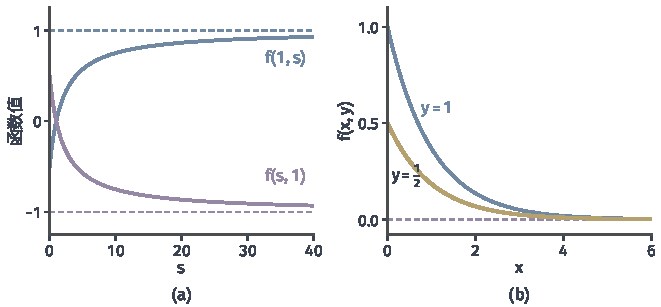
\includegraphics[width=112mm]{figures/05-optimization/07-multiple-criteria-and-nested-optimization/matplotlib/minimax-exchange-fail/figure.pdf}
 \caption{放宽紧性的两种后果。(a)$f=(y-x)/(1+x+y)$在$[0,\infty)^2$上：蓝线$f(1,s)$沿$y=s$趋于蓝色虚线$1$，紫线$f(s,1)$沿$x=s$趋于紫色虚线$-1$，两个次序的值不同。(b)$f=ye^{-x}$：蓝线和黄线分别是$y=1,\frac12$时的截线，都趋于紫色虚线$0$而取不到，值相等但没有鞍点。}
 \label{fig:minimax-exchange-fail}
\end{BookInlineFigure}

最值相等是一个关于数的结论。要从中取出一对点，还必须分别核对$\phi$的最小值和$\psi$的最大值是否达到。

\subsection{鞍点间隙}
\label{sec:minimax-gap}

有了$\phi$和$\psi$，就能给任何一对可行候选打分。这是第~\ref{chap:duality}章“可行点给上界、乘子给下界”的直接推广。

\begin{definition}[鞍点间隙]
\label{def:minimax-gap}
对$(\bm{x},\bm{y})\in\bm{X}\times\bm{Y}$，定义
\begin{equation}
 G(\bm{x},\bm{y})=\sup_{\bm{v}\in\bm{Y}}f(\bm{x},\bm{v})-\inf_{\bm{u}\in\bm{X}}f(\bm{u},\bm{y})=\phi(\bm{x})-\psi(\bm{y}),
 \label{eq:minimax-gap}
\end{equation}
称为\term{鞍点间隙}（saddle gap），其中$\phi(\bm{x})=+\infty$或$\psi(\bm{y})=-\infty$时$G=+\infty$。
\end{definition}

间隙度量的是：固定对方，各自还能改善多少，两边加起来。

\begin{theorem}[间隙是全局证书]
\label{thm:minimax-gap}
对任意$(\bm{x},\bm{y})\in\bm{X}\times\bm{Y}$，只要$G(\bm{x},\bm{y})$有定义，就有$G(\bm{x},\bm{y})\geq\bar{v}-\underline{v}\geq0$，并且
\begin{equation}
 \phi(\bm{x})-\bar{v}\leq G(\bm{x},\bm{y}),\qquad\underline{v}-\psi(\bm{y})\leq G(\bm{x},\bm{y}).
 \label{eq:minimax-gap-bound}
\end{equation}
当$G(\bm{x},\bm{y})$有限时，$G(\bm{x},\bm{y})=0$当且仅当$(\bm{x},\bm{y})$是全局鞍点。
\end{theorem}

\begin{proof}
由定义，$\phi(\bm{x})\geq\bar{v}$，$\psi(\bm{y})\leq\underline{v}$，相减得$G\geq\bar{v}-\underline{v}$，它由式~\eqref{eq:minimax-weak}非负。

式~\eqref{eq:minimax-gap-bound}的第一式等价于$\psi(\bm{y})\leq\bar{v}$，它由$\psi(\bm{y})\leq\underline{v}\leq\bar{v}$得到。第二式等价于$\underline{v}\leq\phi(\bm{x})$，它由$\underline{v}\leq\bar{v}\leq\phi(\bm{x})$得到。

若$G=0$，由上面的不等式，$\phi(\bm{x})=\bar{v}$，$\psi(\bm{y})=\underline{v}$，且$\bar{v}=\underline{v}$，由定理~\ref{thm:minimax-saddle-values}它是全局鞍点。反过来，全局鞍点满足式~\eqref{eq:minimax-saddle-values}，相减为零。
\end{proof}

式~\eqref{eq:minimax-gap-bound}是最有用的部分。它不需要知道$\bar{v}$，就能说出$\bm{x}$的最坏值离最优最多差多少。回到比例松弛，取图~\ref{fig:minimax-relaxed-table}的绿点$(p,q)=(0.8,0.5)$，算得
\[
 \phi(0.8)=\max\{1.2,2.4\}=2.4,\qquad\psi(0.5)=\min\{1,2\}=1.
\]
所以
\[
 G(0.8,0.5)=1.4.
\]
真实的次优量是$\phi(0.8)-\frac32=0.9$，确实不超过$1.4$。

对$f=xy$，$X=Y=[-1,1]$，有
\begin{equation}
 \phi(x)=\lvert x\rvert,\qquad\psi(y)=-\lvert y\rvert,\qquad G(x,y)=\lvert x\rvert+\lvert y\rvert.
 \label{eq:minimax-box-gap}
\end{equation}
这个例子的答案可以直接读出来，后面却会看到，最直接的算法在它上面就会失败。

\paragraph{非紧域上的间隙}
把上面的集合换成$X=Y=\mathbb{R}$，同一个$f=xy$的$\phi(x)$在$x\neq0$时是$+\infty$，于是$G$除了原点处处是$+\infty$。此时$G$虽然没有错，却完全不能区分候选的好坏。

常见的处理是只在一个有界区域$\bm{B}=\bm{B}_{\bm{X}}\times\bm{B}_{\bm{Y}}$上取极值，其中$\bm{B}_{\bm{X}}\subseteq\bm{X}$，$\bm{B}_{\bm{Y}}\subseteq\bm{Y}$，候选在$\bm{B}$内，得到
\begin{equation}
 G_{\bm{B}}(\bm{x},\bm{y})=\sup_{\bm{v}\in\bm{B}_{\bm{Y}}}f(\bm{x},\bm{v})-\inf_{\bm{u}\in\bm{B}_{\bm{X}}}f(\bm{u},\bm{y}).
 \label{eq:minimax-restricted-gap}
\end{equation}

称为\term{限定间隙}（restricted gap）。上确界和下确界的范围变小，所以$G_{\bm{B}}\leq G$。它是真实间隙的下估计，小的$G_{\bm{B}}$不能说明$G$小。

式~\eqref{eq:minimax-local-saddle}正好说明这一点。取$\bm{B}=[-1,1]\times[-1,1]$，候选为原点。在$\bm{B}$内$x^2-\frac14x^4\geq0$，$-y^2\leq0$，所以$G_{\bm{B}}(0,0)=0$。但在整个$X=[-3,3]$上，
\[
 \psi(0)=\min_{\lvert u\rvert\leq3}\Bigl(u^2-\frac14u^4\Bigr)=-11.25,\qquad\phi(0)=0.
\]
所以真实间隙是$11.25$，见图~\ref{fig:minimax-restricted-gap}。局部检验框看不到框外的低谷，零的限定间隙不能当作全局证书。

\begin{BookInlineFigure}
 \centering
 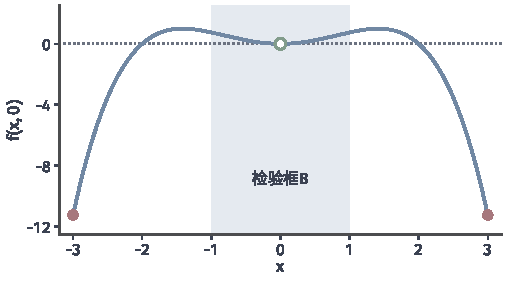
\includegraphics[width=86mm]{figures/05-optimization/07-multiple-criteria-and-nested-optimization/matplotlib/minimax-restricted-gap/figure.pdf}
 \caption{$f(x,y)=x^2-\frac14x^4-y^2$在$y=0$上的截线，$X=[-3,3]$。浅蓝区域是检验框，框内原点（绿色空心点）的值最小，限定间隙为零。红点是框外的真正最小点，值为$-11.25$，真实间隙是$11.25$。}
 \label{fig:minimax-restricted-gap}
\end{BookInlineFigure}

凸凹问题里限定间隙的意义强一些。若$\bm{B}$内含有一个全局鞍点$(\bm{x}^\star,\bm{y}^\star)$，则
\[
 G_{\bm{B}}(\bm{x},\bm{y})\geq f(\bm{x},\bm{y}^\star)-f(\bm{x}^\star,\bm{y})\geq0,
\]
所以它至少是一个非负的度量，只要$\bm{B}$足够大，把解包含在内。这条依赖“$\bm{B}$内含解”这个事实，而这个事实本身需要另外的证据。
